

%%%%%%%%%%%%%%%%%%%%%%%%%%%%%%%%%%%%%%%%%

%----------------------------------------------------------------------------------------
%	PACKAGES AND THEMES
%----------------------------------------------------------------------------------------

\documentclass{beamer}

\mode<presentation> {

% The Beamer class comes with a number of default slide themes
% which change the colors and layouts of slides. Below this is a list
% of all the themes, uncomment each in turn to see what they look like.

%\usetheme{default}
%\usetheme{AnnArbor}
%\usetheme{Antibes}
%\usetheme{Bergen}
%\usetheme{Berkeley}
%\usetheme{Berlin}
%\usetheme{Boadilla}
%\usetheme{CambridgeUS}
%\usetheme{Copenhagen}
%\usetheme{Darmstadt}
%\usetheme{Dresden}
%\usetheme{Frankfurt}
%\usetheme{Goettingen}
%\usetheme{Hannover}
%\usetheme{Ilmenau}
%\usetheme{JuanLesPins}
%\usetheme{Luebeck}
\usetheme{Madrid}
%\usetheme{Malmoe}
%\usetheme{Marburg}
%\usetheme{Montpellier}
%\usetheme{PaloAlto}
%\usetheme{Pittsburgh}
%\usetheme{Rochester}
%\usetheme{Singapore}
%\usetheme{Szeged}
%\usetheme{Warsaw}

% As well as themes, the Beamer class has a number of color themes
% for any slide theme. Uncomment each of these in turn to see how it
% changes the colors of your current slide theme.

%\usecolortheme{albatross}
%\usecolortheme{beaver}
%\usecolortheme{beetle}
%\usecolortheme{crane}
%\usecolortheme{dolphin}
%\usecolortheme{dove}
%\usecolortheme{fly}
%\usecolortheme{lily}
%\usecolortheme{orchid}
%\usecolortheme{rose}
%\usecolortheme{seagull}
%\usecolortheme{seahorse}
%\usecolortheme{whale}
%\usecolortheme{wolverine}

%\setbeamertemplate{footline} % To remove the footer line in all slides uncomment this line
%\setbeamertemplate{footline}[page number] % To replace the footer line in all slides with a simple slide count uncomment this line

%\setbeamertemplate{navigation symbols}{} % To remove the navigation symbols from the bottom of all slides uncomment this line
}
% \definecolor{UBCblue}{rgb}{0.32549, 0.25098, 0.35294} % UBC Blue (primary)
\definecolor{UBCblue}{rgb}{0.0, 0.0, 0.0}
\usecolortheme[named=UBCblue]{structure}
\usepackage{graphicx} % Allows including imageshttps://www.overleaf.com/project/619f79aeb4caa077a85f2fad
\usepackage{booktabs} % Allows the use of \toprule, \midrule and \bottomrule in tables
\usepackage{listings}
\usepackage[vietnamese]{babel}
%----------------------------------------------------------------------------------------
%	TITLE PAGE
%----------------------------------------------------------------------------------------

\title[Seminar ]{Recommendation System} % The short title appears at the bottom of every slide, the full title is only on the title page

\author{20424008 - Dương Mạnh Cường} % 

\institute[UCLA] % Your institution as it will appear on the bottom of every slide, may be shorthand to save space
{
Đại học Khoa Học Tự Nhiên - ĐHQG\\ % Your institution for the title page
\medskip
\textit{Thành phố Hồ Chí Minh} % 
}
\date{} % Date, can be changed to a custom date

\begin{document}

\begin{frame}
\titlepage % Print the title page as the first slide
\end{frame}

\begin{frame}
\frametitle{Nội dung} % Table of contents slide, comment this block out to remove it
\tableofcontents % Throughout your presentation, if you choose to use \section{} and \subsection{} commands, these will automatically be printed on this slide as an overview of your presentation
\end{frame}

%----------------------------------------------------------------------------------------
%	PRESENTATION SLIDES
%----------------------------------------------------------------------------------------

%------------------------------------------------
\section{Bài toán mở đầu} % Sections can be created in order to organize your presentation into discrete blocks, all sections and subsections are automatically printed in the table of contents as an overview of the talk
%------------------------------------------------

\subsection{Mục tiêu} % A subsection can be created just before a set of slides with a common theme to further break down your presentation into chunks
\subsection{Các phương pháp truyền thống} % A subsection can be created just before a set of slides with a common theme to further break down your presentation into chunks
%------------------------------------------------
\section{Thống kê} % Sections can be created in order to organize your presentation into discrete blocks, all sections and subsections are automatically printed in the table of contents as an overview of the talk
%------------------------------------------------
\section{Ứng dụng} % Sections can be created in order to organize your presentation into discrete blocks, all sections and subsections are automatically printed in the table of contents as an overview of the talk
%------------------------------------------------
\section{4.	Các loại tấn công chung:} % Sections can be created in order to organize your presentation into discrete blocks, all sections and subsections are automatically printed in the table of contents as an overview of the talk
%------------------------------------------------
\section{5.	Biện pháp đối phó:} % Sections can be created in order to organize your presentation into discrete blocks, all sections and subsections are automatically printed in the table of contents as an overview of the talk
%------------------------------------------------
\begin{frame}
\frametitle{Nguy cơ, mối đe dọa, lỗ hổng}
Nguy cơ, đe dọa và lỗ hổng luôn đi chung với nhau.\\
+ Nguy cơ: thứ gì đó tệ có thể xảy ra.\\
+ Đe dọa: hành động gây nguy hiểm cho hệ thống và tài nguyên.\\
+ Lỗ hổng: có thể bị khai thác từ 1 tác nhân đe dọa nào đó.\\
Không thể loại bỏ nguy cơ nhưng có thể ngăn ngừa các lỗ hổng bảo mật.	Chìa khóa để bảo vệ tài nguyên khỏi các nguy cơ của cuộc tấn công là loại bỏ hoặc đánh dấu các lỗ hổng càng nhiều càng tốt.\\
Có thể tìm ra nhiều mối đe dọa cũng như lỗ hổng bảo mật trong các tài nguyên cơ sở hạ tầng IT. Bảng sau liệt kê một số lỗi chung thường xảy ra khi sử dụng các cơ sở hạ tầng IT dưới đây.

\end{frame}

%------------------------------------------------
%------------------------------------------------
\begin{frame}
\begin{figure}[h]
\centering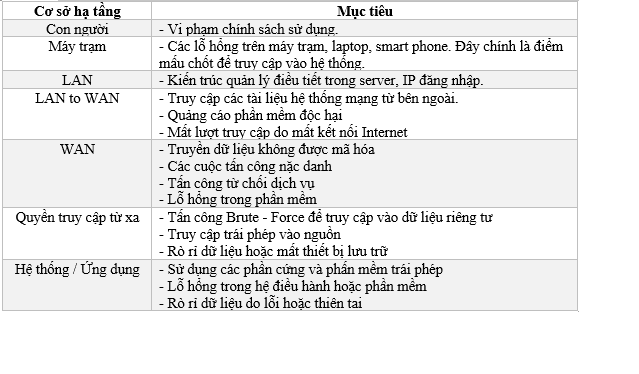
\includegraphics[width=1\linewidth]{images/pic1.png}
\end{figure}
\end{frame}

%------------------------------------------------

\begin{frame}
\frametitle{Nguy cơ, mối đe dọa, lỗ hổng}
\text{Các mối đe doa phổ biến}\\
\begin{itemize}
\item Phần mểm độc hại.
\item Lỗi phần cứng hoặc phần mềm.
\item Tấn công từ nội bộ bên trong.
\item Mất cắp thiết bị.
\item Tấn công từ bên ngoài.
\item Thiên tai.
\item Gián điệp.
\item Khủng bố.

\end{itemize}
\end{frame}

%------------------------------------------------

\begin{frame}
\frametitle{Các loại đe dọa cho hệ thống}
\begin{block}{ Mối đe dọa tiết lộ thông tin}
 Tiết lộ xảy ra bất cứ khi nào người dùng trái phép truy cập thông tin cá nhân hoặc bí mật được lưu trữ trên tài nguyên mạng hoặc trong khi nó đang truyền tải giữa các tài nguyên mạng. . Hai kỹ thuật sau được kẻ tấn công sử dụng trái phép có được hoặc sửa đổi dữ liệu:
 \begin{itemize}
\item Sabotage (Phá hoại ngầm): Phá hủy tài sản hoặc cản trở  những hoạt động bình thường.
\item Espionage (Gián điệp): là hành động do thám để có được thông tin bí mật, điển hình là để hỗ trợ cho quốc gia khác.
\end{itemize}
\end{block}

\begin{block}{Mối đe dọa thay đổi thông tin}
Vi phạm tính toàn vẹn thông tin. Kiểu tấn công này làm hại hệ thống bằng cách thực hiện các thay đổi trái phép dữ liệu trên một hệ thống do cố ý hoăc vô ý. Thay đổi có chủ ý thường là độc hại. 
\end{block}

\end{frame}

%------------------------------------------------
\begin{frame}
\frametitle{}
\begin{block}{ - Mối đe dọa từ chối và phá hủy}
 
 \begin{itemize}
\item Các mối đe dọa từ chối hoặc phá hủy làm cho tài sản hoặc tài nguyên không có sẵn hoặc không thể sử dụng được.
\item Vi phạm nguyên lý sẵn có của bảo mật thông tin.
\item Một cuộc tấn công từ chối hoặc phá hủy thành công khi nó ngăn người dùng được ủy quyền truy cập tài nguyên tạm thời hoặc vĩnh viễn.
\item Tấn công DoS là một ví dụ về mối đe dọa từ chối hoặc phá hủy.
\end{itemize}
\end{block}
\end{frame}

%------------------------------------------------

\begin{frame}
\frametitle{Tấn công khai thác lỗ hổng}

\textbf{Các cuộc tấn công có thể bao gồm cả 4 phương thức sau:}
\begin{enumerate}
\item Giả mạo: tạo ra một số mánh khóe để người dùng không nghi ngờ hệ thống đã bị tấn công.
\item Chặn thông tin: Liên quan đến việc nghe lén các truyền và chuyển hướng chúng để sử dụng trái phép.
\item Gián đoạn thông tin: Gây ra sự gián đoạn trong một kênh truyền thông, ngăn chặn việc truyền dữ liệu.
\item Thay đổi thông tin: thay đổi dữ liệu có trong các đường truyền hoặc tập tin.
\end{enumerate}

\textbf{2 nhóm tấn công:}
\begin{enumerate}
\item Tấn công nhằm thay đổi các dữ liệu.
\item Tấn công nhằm nghe lén và theo dõi các dữ liệu.
\end{enumerate}
\end{frame}
%------------------------------------------------
\begin{frame}
\frametitle{Các tấn công độc hại}
    \begin{block}{Birthday attacks:}
         \begin{itemize}
    \item Tấn công Ngày sinh là một loại tấn công mật mã dựa trên sự khai thác vấn đề Ngày sinh (Birthday problem)- một hiện tượng xác suất tạo ra nghịch lý đối với cảm giác của con người, do vậy còn được gọi là “Nghịch lý Ngày sinh”(Birthday paradox). Áp dụng lí thuyết xác suất thống kê, giả sử trong 1 phòng có 23 người ngẫu nhiên, xác suất có ít nhất  2 người trùng ngày sinh là 50\%.
    \item Công thức tổng quát để tính xác suất có ít nhất 2 người trùng ngày sinh trong n người ngẫu nhiên:
    \begin{figure}[h]
    \centering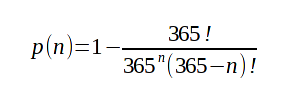
\includegraphics[width=0.4\linewidth]{images/bday.png}
    \end{figure}
    \item Với n = 70 người ngẫu nhiên, p(n) ~ 99\%, nghĩa là gần như chắc chắn trong 70 người ngẫu nhiên có 2 người trùng ngày sinh.
\end{itemize}
    \end{block}
\end{frame}

%-----------------------------------------------
\begin{frame}
\frametitle{Các tấn công độc hại}
    \begin{block}{Brute – force:}
         \begin{itemize}
    \item Kẻ tấn công sẽ thử các mật khẩu khác nhau tr6en một hệ thống cho đến khi thành công. 
    \item Kiểu tấn công này không có kỹ năng hay sự lén lút chỉ dùng vũ lực mà cuối cùng phá vỡ mã.
    \item Với máy tính quy mô lớn ngày nay, có thể thử hàng triệu kết hợp mật khẩu trong một khoảng thời gian ngắn. Nếu đủ thời gian và đủ máy tính, có thể bẻ khóa hầu hết các thuật toán..
\end{itemize}
    \end{block}
\end{frame}

%-----------------------------------------------
\begin{frame}
\frametitle{Các tấn công độc hại}
    \begin{block}{Dictionary password attacks}
         \begin{itemize}
    \item Là một cuộc tấn công đơn giản dựa vào người dùng thực hiện các lựa chọn mật khẩu kém. Chương trình bẻ khóa mật khẩu đơn giản sẽ lấy tất cả các từ trong tệp từ điển và cố gắng đăng nhập bằng cách nhập từng mục từ điển làm mật khẩu.
    \item Một chính sách mật khẩu thực thi mật khẩu phức tạp là cách bảo vệ tốt nhất đối với kiểu tấn công từ điển mật khẩu. Người dùng nên tạo mật khẩu gồm một tổ hợp các chữ cái và số và mật khẩu không được bao gồm bất kỳ thông tin cá nhân nào về người dùng.
\end{itemize}
    \end{block}
\end{frame}
%------------------------------------------------
\begin{frame}
\frametitle{Các tấn công độc hại}
    \begin{block}{IP Address Spoofing:}
         \begin{itemize}
    \item Kĩ thuật này áp dụng khi một máy bên ngoài hệ thống muốn liên kết vào hệ thống đó mà không thông báo trước. Máy tính bên ngoài phải giành được 1 IP để đánh lừa hệ thống. Khi đã xâm nhập thành công, hacker có thể thực hiện tấn công từ chối dịch vụ để làm máy chủ bị nghẽn. 
\end{itemize}
    \end{block}
\end{frame}
%------------------------------------------------
\begin{frame}
\frametitle{Các tấn công độc hại}
\begin{block}{ Hijacking: }
    Là một kiểu tấn công trong đó kẻ tấn công chiếm quyền kiểm soát phiên giữa hai máy và giả mạo là một trong số chúng. Có một số loại Hijacking:
 \begin{itemize}
\item Man-in-the-middle hijacking: Kẻ tấn công sử dụng một chương trình để kiểm soát kết nối bằng cách giả mạo như mỗi đầu của kết nối.
\item Browser/ URL hijacking: Chiếm quyền điều khiển trình duyệt hoặc URL Kẻ tấn công có thể sử dụng cuộc tấn công này để lừa đảo để lừa người dùng cung cấp thông tin cá nhân như mật khẩu.(Phising).
\item Session Hijacking:  Là hình thức tấn công vào phiên làm việc giữa client và server bằng cách đánh cắp cookie của người sử dụng sau khi họ đã qua bước xác thực với máy chủ sau đó sẽ chiếm quyền điều khiển của phiên làm việc này.
\end{itemize}
    \end{block}
\end{frame}
%------------------------------------------------
\begin{frame}
\frametitle{Các tấn công độc hại}
    \begin{block}{Replay Attacks:}
         \begin{itemize}
    \item Tấn công mạng lưới trong đó các thực thể độc hại chặn và lặp lại việc truyền tải một dữ liệu hợp lệ đi vào trong mạng lưới. Nhờ có tính hợp lệ của dữ liệu ban đầu (thường đến từ người dùng đã được cấp quyền), các giao thức bảo mật của mạng lưới sẽ xử lý vụ việc tấn công này chỉ giống như một hình thức truyền tải dữ liệu thông thường. Do các tệp tin ban đầu  đã bị ngăn chặn và được truyền tải lại nguyên văn nên hacker thực hiện vụ tấn công sẽ không cần giải mã chúng.
\end{itemize}
    \end{block}
\end{frame}
%------------------------------------------------

\begin{frame}
\frametitle{Các tấn công độc hại}
    \begin{block}{Main in the middle:}
         \begin{itemize}
    \item Hành động xen giữa cuộc giao tiếp giữa 2 thiết bị mà chúng không hề biết. 2 thiết bị cho rằng đang giao tiếp trong môi trường riêng tư, nhưng thực ra các trao đổi giữa 2 bên lại bị bên thứ 3 nghe lén và thu thập được. Trong kiểu tấn công này, kẻ tấn công chặn tin nhắn giữa hai bên trước khi chuyển chúng đến đích dự định.
    \begin{figure}[h]
    \centering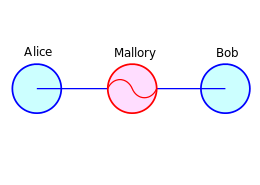
\includegraphics[width=0.4\linewidth]{images/man-in-middle.png}
    \end{figure}
\end{itemize}
    \end{block}
\end{frame}
%------------------------------------------------
\begin{frame}
\frametitle{Các tấn công độc hại}
    \begin{block}{Masquerading:}
         \begin{itemize}
    \item Máy tính và người dùng giả vờ là một máy tính hoặc người dùng khác.
    \item Các cuộc tấn công giả trang thường bao gồm một trong các hình thức tấn công hoạt động khác, chẳng hạn như giả mạo địa chỉ IP hoặc phát lại. Kẻ tấn công có thể nắm bắt các chuỗi xác thực và sau đó phát lại chúng để đăng nhập lại vào một ứng dụng hoặc hệ điều hành.
\end{itemize}
    \end{block}
\end{frame}
%------------------------------------------------

\begin{frame}
\frametitle{Eavesdropping}
	\begin{block}{}
		Tạo ra các gói tin có địa chỉ IP giả mạo không là địa chỉ máy gửi gói tin
	\end{block}
	\begin{block}{}
		Vượt qua các kiểm soát về nguồn gốc địa chỉ IP.
	\end{block}
	\begin{block}{}
			Phục vụ các mô hình tấn công khác.
			\begin{itemize}
                \item Tấn công về phiên Tấn công về session.
                \item Tấn công kiểu phản xạ.
            \end{itemize}
	\end{block}
	\begin{block}{}
		Giải pháp:
			\begin{itemize}
                \item Không sử dụng xác thực là địa chỉ IP.
                \item Phát hiện các bất thường về kết nối Phát hiện các bất thường về kết nối mạng.
            \end{itemize}
	\end{block}
\end{frame}

%------------------------------------------------
\begin{frame}
\frametitle{Các tấn công độc hại}
    \begin{block}{Social Engineering:}
         \begin{itemize}
    \item Là kỹ thuật tác động đến con người, nhằm mục đích lấy được thông tin hoặc đạt được một mục đích mong muốn. 
    \item Dựa trên nền tảng là điểm yếu tâm lý, nhận thức sai lầm của con người về việc bảo mật thông tin, sử dụng sự ảnh hưởng và thuyết phục để đánh lừa người dùng nhằm khai thác các thông tin có lợi cho cuộc tấn công, hoặc thuyết phục nạn nhân thực hiện một hành động nào đó
    \item Tiến hành khai thác các thói quen tự nhiên của người dùng, hơn việc khai thác các lỗ hổng bảo mật của hệ thống. Người dùng được trang bị kém về kiến thức bảo mật sẽ là cơ sở để tin tặc thực hiện tấn công.
\end{itemize}
    \end{block}
\end{frame}
%------------------------------------------------
%------------------------------------------------
\begin{frame}
\frametitle{Các tấn công độc hại}
    \begin{block}{Phreaking:}
         \begin{itemize}
    \item Phreaking là nghệ thuật khai thác lỗi và trục trặc tồn tại trong hệ thống điện thoại.
    \item •	Bằng cách phreaking, những người này có thể thực hiện một cuộc gọi dài miễn phí hoặc thậm chí là thực hiện cuộc gọi trên máy của người khác.
\end{itemize}
    \end{block}
\end{frame}
%------------------------------------------------
\begin{frame}
\frametitle{Các tấn công độc hại}
    \begin{block}{Phishing}
         \begin{itemize}
    \item Kẻ tấn công cố gắng lừa nạn nhân cung cấp thông tin cá nhân thông qua email hoặc tin nhắn tức thời. 
    \item Thông điệp hướng dẫn nạn nhân cung cấp thông tin được yêu cầu hoặc nhấp vào một liên kết được cung cấp trong tin nhắn  nạn nhân của một trang web giả mạo trông giống hệt với chính thức nhưng trên thực tế thuộc về kẻ lừa đảo. Thông tin cá nhân đã nhập vào trang web này đi trực tiếp đến kẻ lừa đảo.
\end{itemize}
    \end{block}
\end{frame}
%------------------------------------------------

\begin{frame}
\frametitle{Các tấn công độc hại}
    \begin{block}{Pharming}
         \begin{itemize}
    \item Một loại tấn công khác nhằm tìm cách lấy thông tin tài chính cá nhân hoặc riêng tư thông qua việc giả mạo tên miền. 
\end{itemize}
    \end{block}
\end{frame}
%------------------------------------------------
%------------------------------------------------
\begin{frame}
\frametitle{Phần mềm độc hại}
    \begin{block}{Phreaking:}
         \begin{itemize}
    \item Phreaking là nghệ thuật khai thác lỗi và trục trặc tồn tại trong hệ thống điện thoại.
    \item Bằng cách phreaking, những người này có thể thực hiện một cuộc gọi dài miễn phí hoặc thậm chí là thực hiện cuộc gọi trên máy của người khác.
\end{itemize}
    \end{block}
\end{frame}

%------------------------------------------------

\begin{frame}
\frametitle{Phần mềm độc hại}
    \begin{block}{Cương trình lây nhiễm:}
         \begin{itemize}
    \item Cố gắng sao chép bản thân sang các máy tính khác. Mục đích chính của nó là để thực hiện một hướng dẫn tấn công của kẻ tấn công vào các mục tiêu mới. Bao gồm:Virues, worms
        \end{itemize}
    \end{block}
    \begin{block}{Cương trình ẩn:}
         \begin{itemize}
    \item Ngầm phá hủy, thu thập thông tin trên thiết bị mà không để bị phát hiện. Bao gồm: Trojan horses,Rootkits, spyware.
        \end{itemize}
    \end{block}
\end{frame}


%------------------------------------------------

\begin{frame}
\frametitle{Phần mềm độc hại}
	\begin{block}{Viruses}
	Chương trình thâm nhập vào máy tính và tự nhân lên mà không có tác động của người dùng. Có nhiều loại virus khác nhau dựa trên mức độ phá hoại và mục tiêu của nó. 
	\end{block}
	\begin{block}{Worms}
    Là môt dạng kết hợp giữa sức phá hoại, lây lan của virus và tính âm thầm của Trojan. 1 số các worm tồn tại như 1 tập tin, số khác nằm trong bộ nhớ máy tính.
	\end{block}
	\begin{block}{Trojan Horses}
	Trojan không tự nhân bản được.Bên ngoài trông có vẻ là phần mềm có ích, nhưng nó chỉ tạo lớp ỏ bên ngoài để thâm nhập và phá hủy từ bên trong. 
	\end{block}
\end{frame}

%------------------------------------------------
\begin{frame}
\frametitle{Phần mềm độc hại}
	\begin{block}{Rootkits}
   Là biến thể mới của phần mềm độc hại, được thiết kế để ẩn mình và vượt qua được nhiều phần mềm bảo vệ. Cần các phần mềm đủ mạnh mới diệt được nó.
	\end{block}
	\begin{block}{Spyware}
    Được đóng gói như một thành phần ẩn của phần mềm miễn phí hoặc phần mềm chia sẻ các chương trình mà người dùng tải xuống từ Internet, tương tự như Trojan. Nó cũng có thể lây lan thông qua trao đổi tập tin ngang hàng
	\end{block}
\end{frame}
%------------------------------------------------
\begin{frame}
\frametitle{Các loại tấn công phổ biến}
	\begin{block}{Tấn công vào tính sẵn sàng}
    Làm ảnh hưởng hoặc tê liệt hoàn  toàn các hoạt động tương tác giữa hệ thống với người dùng. 
	\end{block}
	\begin{block}{Tấn công vào con người}
   Đánh vào sự tò mò hoặc ép người dùng phải tiết lộ thông tin hay nhấp vào 1 đường link chứa mã độc nào đó hay dc gửi từ 1 mai không xác định.
	\end{block}
	\begin{block}{Tấn công vào hệ thống IT}
	Xâm nhập sử dụng tài nguyên trái phép, sửa hoặc xóa các dữ liệu. 
	\end{block}
\end{frame}

%------------------------------------------------

\begin{frame}
\frametitle{Social Engineering Attacks}
  •	Dưới đây là tóm tắt về các cuộc tấn công kỹ thuật xã hội
     \begin{itemize}
    \item Authority: Sử dụng một vị trí của chính quyền để ép buộc hoặc thuyết phục một cá nhân tiết lộ thông tin.
    \item Đồng thuận / bằng chứng xã hội: Dựa vào việc mà mọi người khác đã và đang thực hiện.rằng nó ổn hoặc có thề chấp nhận.
    \item Dumpsters-diving: Tìm kiếm những mảnh giấy có thể chứa dữ liệu nhạy cảm hoặc dữ liệu riêng tư để lấy cắp danh tính
    \item Hoaxes: Tạo một lừa đảo hoặc nhận thức sai lầm để khiến một cá nhân làm điều gì đó hoặc tiết lộ thông tin.
    \item Impersonation: Giả vờ là một người khác.
    \item Khẩn cấp: Sử dụng khẩn cấp hoặc một tình huống căng thẳng khẩn cấp để khiến ai đó làm gì đó hoặc tiết lộ thông tin.
    \item Vishing: Thực hiện một cuộc tấn công lừa đảo qua điện thoại để lấy thông tin cá nhân sử dụng sự ép buộc bằng lời nói và thuyết phục.
\end{itemize}
\end{frame}

%------------------------------------------------

\begin{frame}
\frametitle{Wireless network attacks }
  •	Các dạng của cuộc tấn công mạng không dây:
     \begin{itemize}
    \item Bluejacking: Chiếm quyền kiểm soát giữa thiết bị Bluetooth và smartphone.
    \item Bluesnarfing: Nghe lén thông tin giữa các thiết bị Bluetooth
    \item Evil twin: Giả mạo 1 mạng mục tiêu nào đó, chuyển hướng thiết bị muốn kết nối vào mạng đó sang 1 nơi chuẩn bị trước và yêu cầu nhập lại mật khẩu của mạng thật, khi đó sẽ chiếm dc mật khẩu của mạng thật.
    \item Jamming/interference: gửi tần số vô tuyến cùng tần số với các điểm truy cập mạng gây nghẽn mạng.
    \item Impersonation: Giả vờ là một người khác.
    \item Near field communication attack: NFC: xen giữa giao tiếp NFC giữa 2 smartphone.
    \item Packet sniffing: Bắt các gói IP khỏi mạng không dây và phân tích TCP / IP dữ liệu gói bằng cách sử dụng một công cụ như Wireshark®..
\end{itemize}
\end{frame}

%------------------------------------------------

\begin{frame}
\frametitle{Web Aplication acttacks}
 
     \begin{itemize}
    \item Thực thi mã tùy ý / từ xa: Có được quyền truy cập đặc quyền hoặc quyền quản trị hệ thống truy cập, kẻ tấn công có thể chạy các lệnh hoặc thực hiện một lệnh theo ý muốn trên điều khiển hệ thống từ xa.
    \item Bufferred overflow: Cố gắng đẩy nhiều dữ liệu hơn khả năng lưu trữ để thay đổi hành vi của chương trình dẫn đến các hiệu ứng không muốn hoặc ghi đè địa chỉ trả về.

    \item Cross-site scripting (XSS): Thêm script vào máy chủ ứng dụng web để chuyển hướng tấn công trở lại máy khác.
    \item SQL Injection:  Thêm các lệnh sql để lấy thông tin và dữ liệu trong cơ sở dữ liệu SQL phía back-end.
    \item Watering-hole attack: Lôi kéo người dùng đến một trang web thường truy cập trên đó đã được cài mã độc hoặc phần mềm độc hại với hy vọng người dùng sẽ kích hoạt tấn công với một cú nhấp chuột không biết.
\end{itemize}
\end{frame}
%------------------------------------------------

\begin{frame}
\frametitle{Biện pháp ngăn ngừa}
     \begin{itemize}
    \item Tạo một chương trình giáo dục (nhận thức bảo mật thông tin) để ngăn người dùng khỏi cài đặt phần mềm độc hại trên hệ thống.
    \item Đăng các bản tin thường xuyên về các vấn đề về phần mềm độc hại.
    \item Không bao giờ chuyển tệp từ một nguồn không xác định hoặc không đáng tin trừ khi máy tính có một tiện ích chống phần mềm độc hại được cài đặt.
    \item Cài đặt phần mềm chống phần mềm độc hại, đảm bảo phần mềm và dữ liệu hiện tại và lên lịch quét phần mềm độc hại thường xuyên.
    \item Sử dụng quy trình xác thực và đăng nhập an toàn.
\end{itemize}

\end{frame}


%------------------------------------------------


\begin{frame}
\frametitle{Các biện pháp ngăn ngừa}
     \begin{itemize}
    \item Một số phần mềm anti malware: BitDefender, Kaspersky Anti-Virus, Webroot Antivirus, Norton Antivirus,…
    \item Bảo vê hệ thống với tường lửa:  Có rất nhiều giải pháp tường lửa có sẵn. Các nhà cung cấp tường lửa nổi bật bao gồm: Palo Alto Networks, Cisco System, SonicWALL,…
    
\end{itemize}

\end{frame}
%------------------------------------------------
\begin{frame}[fragile]
    \begin{verbatim}
    print("helo")
    print("helo")
    print("helo")
    print("helo")
    print("helo")
    print("helo")
    print("helo")
    print("helo")
    print("helo")
    print("helo")
    print("helo")
    print("helo")
    print("helo")
    print("helo")
    print("helo")
    print("helo")
    print("helo")
    print("helo")
    print("helo")
    print("asdadadelo")

    print("helo")

    \end{verbatim}
    \end{frame}






\begin{frame}
\Huge{\centerline{The End}}
\end{frame}

%----------------------------------------------------------------------------------------

\end{document} 